%!TEX TS-program = xelatex
\documentclass[12pt, a4paper, oneside]{article}

\usepackage{amsmath,amsfonts,amssymb,amsthm,mathtools}  % пакеты для математики

\usepackage[utf8]{inputenc} % задание utf8 кодировки исходного tex файла
\usepackage[british,russian]{babel} % выбор языка для документа

\usepackage{fontspec}         % пакет для подгрузки шрифтов
\setmainfont{Helvetica}   % задаёт основной шрифт документа

% why do we need \newfontfamily:
% http://tex.stackexchange.com/questions/91507/
\newfontfamily{\cyrillicfonttt}{Helvetica}
\newfontfamily{\cyrillicfont}{Helvetica}
\newfontfamily{\cyrillicfontsf}{Helvetica}

\usepackage{unicode-math}     % пакет для установки математического шрифта
\setmathfont{Neo Euler}      % шрифт для математики
% \setmathfont[math-style=ISO]{Asana Math}
% Можно делать смену начертания с помощью разных стилей

% Конкретный символ из конкретного шрифта
% \setmathfont[range=\int]{Neo Euler}

%%%%%%%%%% Работа с картинками %%%%%%%%%
\usepackage{graphicx}                  % Для вставки рисунков
\usepackage{graphics}
\graphicspath{{images/}{pictures/}}    % можно указать папки с картинками
\usepackage{wrapfig}                   % Обтекание рисунков и таблиц текстом

%%%%%%%%%%%%%%%%%%%%%%%% Графики и рисование %%%%%%%%%%%%%%%%%%%%%%%%%%%%%%%%%
\usepackage{tikz, pgfplots}  % язык для рисования графики из latex'a

%%%%%%%%%% Гиперссылки %%%%%%%%%%
\usepackage{xcolor}              % разные цвета

\usepackage{hyperref}
\hypersetup{
	unicode=true,           % позволяет использовать юникодные символы
	colorlinks=true,       	% true - цветные ссылки, false - ссылки в рамках
	urlcolor=blue,          % цвет ссылки на url
	linkcolor=black,          % внутренние ссылки
	citecolor=green,        % на библиографию
	pdfnewwindow=true,      % при щелчке в pdf на ссылку откроется новый pdf
	breaklinks              % если ссылка не умещается в одну строку, разбивать ли ее на две части?
}


\usepackage{todonotes} % для вставки в документ заметок о том, что осталось сделать
% \todo{Здесь надо коэффициенты исправить}
% \missingfigure{Здесь будет Последний день Помпеи}
% \listoftodos --- печатает все поставленные \todo'шки

\usepackage{enumitem} % дополнительные плюшки для списков
%  например \begin{enumerate}[resume] позволяет продолжить нумерацию в новом списке

\usepackage[paper=a4paper, top=20mm, bottom=15mm,left=20mm,right=15mm]{geometry}
\usepackage{indentfirst}       % установка отступа в первом абзаце главы

\usepackage{setspace}
\setstretch{1}  % Межстрочный интервал
\setlength{\parskip}{4mm}   % Расстояние между абзацами
% Разные длины в латехе https://en.wikibooks.org/wiki/LaTeX/Lengths


\usepackage{xcolor} % Enabling mixing colors and color's call by 'svgnames'

\definecolor{MyColor1}{rgb}{0.2,0.4,0.6} %mix personal color
\newcommand{\textb}{\color{Black} \usefont{OT1}{lmss}{m}{n}}
\newcommand{\blue}{\color{MyColor1} \usefont{OT1}{lmss}{m}{n}}
\newcommand{\blueb}{\color{MyColor1} \usefont{OT1}{lmss}{b}{n}}
\newcommand{\red}{\color{LightCoral} \usefont{OT1}{lmss}{m}{n}}
\newcommand{\green}{\color{Turquoise} \usefont{OT1}{lmss}{m}{n}}

\usepackage{titlesec}
\usepackage{sectsty}
%%%%%%%%%%%%%%%%%%%%%%%%
%set section/subsections HEADINGS font and color
\sectionfont{\color{MyColor1}}  % sets colour of sections
\subsectionfont{\color{MyColor1}}  % sets colour of sections

%set section enumerator to arabic number (see footnotes markings alternatives)
\renewcommand\thesection{\arabic{section}.} %define sections numbering
\renewcommand\thesubsection{\thesection\arabic{subsection}} %subsec.num.

%define new section style
\newcommand{\mysection}{
	\titleformat{\section} [runin] {\usefont{OT1}{lmss}{b}{n}\color{MyColor1}} 
	{\thesection} {3pt} {} } 


%	CAPTIONS
\usepackage{caption}
\usepackage{subcaption}
%%%%%%%%%%%%%%%%%%%%%%%%
\captionsetup[figure]{labelfont={color=Turquoise}}

\usepackage[normalem]{ulem}  % для зачекивания текста

\pagestyle{empty}

\usepackage{float}

\begin{document}
	
\section*{Факультатив: Оформление документов в \LaTeX} 

\todo[inline]{Курс рекомендуется всем, кто хотел бы узнать про то, что такое \LaTeX{ } вне зависимости от курса.  Все материалы, используемые в курсе и логи семинаров прошлых лет можно найти на страничке курса на Github: \url{https://fulyankin.github.io/LaTeX/}}

\subsection*{Что за лавртхех?}

\LaTeX{ } ---  штука, про которую многие слышали, но боялись спросить.  \LaTeX{ } --- это издательская система, позволяющая делать красивые документы. Как word, но с большими возможностями и меньшей болью. Чем больше размер документа, который вам нужно сделать, тем меньше боли вы испытываете. А ещё ваш текст выглядит прямо как в книгах! 

В \LaTeX{ } довольно просто оформить диплом по ГОСТ.  Обычно люди, которые пишут диплом в word, довольно сильно страдают от обилия боли. Это подтверждает рисунок 1. Особенно во время нормоконтроля. Обычно при внесении в большой документ небольших изменений, съезжало по 20 табличек. Их приходилось выправлять руками.  Чат нашего курса взрывался от негодования. При этом пять бравых ребят, делавших диплом в \LaTeX{}, прошли через всё это с минимальными страданиями. 


\begin{figure}[H]
	\begin{center}
		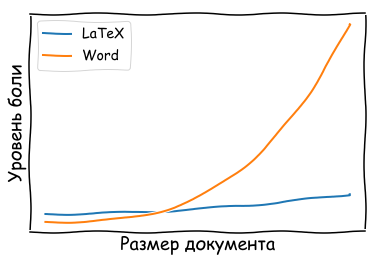
\includegraphics[scale=0.8]{latex.png}\label{pic:1}
	\end{center}
\end{figure}

Я вовсе не говорю, что при изучении \LaTeX{}, записавшимся на курс, не придётся страдать. Однако, если вы посмотрите ещё раз на рисунок  1, вы поймёте, что в асимптотике ваши страдания сократятся. 

\subsection*{Идеология курса}

Курс идёт 8 недель.  Каждую неделю по две пары. Работаем в Xe\LaTeX{}.   Занятия полупрактические. Часть времени я показываю как работают какие куски кода, часть времени мы вместе делаем практические задачи. Часть задач связана с оформлением НИРа. Зачёт выдаётся, если выполнено 70\% заданий. На семинаре в аудитории находится 3-4 человека, которые хорошо знают \LaTeX{}. Если у вас возникают проблемы, мы совместно их обсуждаем. Если вы застопорились, зовите одного из нас! Если есть проблемы, говорите нам о них! У нас нельзя молчать! 

\subsection*{Примерный план занятий} 
 
 \begin{enumerate}
 	\item Обо всём и ни о чём!  Введение в \LaTeX{}.  Мотивация изучать \LaTeX{}. Немного о разных движках (PdfTex, XeTeX и т.д.), что такое юникод и немного подробнее о шрифтах. Математика в \LaTeX{}. В \LaTeX{ } прямо из Wolfram. 
 	\item Рисунки и таблицы в \LaTeX{}. В \LaTeX{ } прямо из Exсel. Безумно красивая графика в TikZ Великая и могучая Geogebra.
 	\item Свои команды и макросы. Оформление документа в целом.
 	\item Преамбула для души и преамбула по ГОСТ.
 	\item Список литературы, biblatex, автоматические ссылки.
 	\item R + \LaTeX{} --- самая мощная связка в мире! Правильное оформление эконометрики. Из R да прямо в НИР. Сбор одного файла из многих разных. 
 	\item R + \LaTeX{} --- продолжаем разговор! Автоматизация создания документов. Как создать 100 красивых анкет для игры в киллера в один клик?
 	\item Презентации в \LaTeX{} --- большая боль или чувство стиля?  Пакет для оформления кода. Что такое Markdown, другие важные мелочи.
  \end{enumerate}
 
 \subsection*{Описание факультатива было долгим, вы заслужили ещё один мем} 
 
 \begin{figure}[H]\label{pic:2}
 	\begin{center}
 		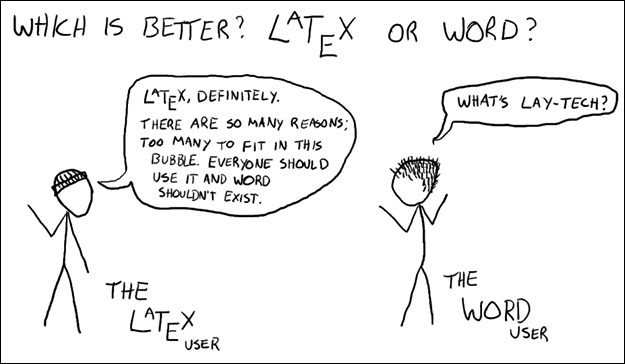
\includegraphics[scale=0.7]{joke_2.png}
 	\end{center}
 \end{figure}








\end{document} 
